%%%%%%%%%%%%%%%%%%%%%%%%%%%%%%%%%%%%
% This is the template for submission to MICRO 2019
% The cls file is modified from 'sig-alternate.cls'
%%%%%%%%%%%%%%%%%%%%%%%%%%%%%%%%%%%%

\documentclass{sig-alternate}
\usepackage{mathptmx} % This is Times font

\usepackage{graphicx}
\usepackage{array}
\usepackage{fancyhdr}
\usepackage[normalem]{ulem}
\usepackage[hyphens]{url}
\usepackage[sort,nocompress]{cite}
\usepackage[final]{microtype}
\usepackage{flushend}
% Always include hyperref last
\usepackage[bookmarks=true,breaklinks=true,letterpaper=true,colorlinks,linkcolor=black,citecolor=blue,urlcolor=black]{hyperref}
\graphicspath{{images/}}
% Ensure letter paper
\pdfpagewidth=8.5in
\pdfpageheight=11.5in

\fancypagestyle{firstpage}{
  \fancyhf{}
  \renewcommand{\headrulewidth}{0pt}
  \fancyhead[C]{\vspace{15pt}\normalsize{CS622A : Advanced Computer Architecture
      -- Fall Semester 2019-20, IIT Kanpur}} 
  \fancyfoot[C]{\thepage}
}

\pagenumbering{arabic}

%%%%%%%%%%%---SETME-----%%%%%%%%%%%%%
%%%%%%%%%%%%%%%%%%%%%%%%%%%%%%%%%%%%%
\title{\vspace{-1ex}Hardware assisted Cache Prefetching Techniques\vspace{-4ex}}
\author{\parbox{3 in}{\centering Aditya Rohan
        \thanks{Both authors contributed equally to this research.}\\ 
        \vspace{2pt}
        IIT Kanpur, 160053\\
        \vspace{1pt}
        {\tt\large raditya@iitk.ac.in}}
        \hspace*{ 0.2 in}
        \parbox{3 in}{ \centering Aniket Pandey
        \footnotemark[1]\\
        \vspace{2pt}
        IIT Kanpur, 160113\\
        \vspace{1pt}
        {\tt\large aniketp@iitk.ac.in}}
        \hspace*{ 0.2 in}\vspace{2ex}}

\begin{document}
\maketitle
\thispagestyle{firstpage}
\pagestyle{plain}



%%%%%% -- PAPER CONTENT STARTS-- %%%%%%%%

\begin{abstract}

This document is intended to serve as a sample for submissions to the 52nd International Symposium on Microarchitecture (MICRO), 2019. We provide some guidelines that authors should follow when submitting papers to the conference.  This format is derived from the ACM sig-alternate.cls file, and is used with an objective of keeping the submission version similar to the camera-ready version.

\end{abstract}

\section{Introduction}

This document provides instructions for submitting papers to the ${52}^{nd}$ International Symposium on Microarchitecture (MICRO), 2019.  In an effort to respect the efforts of reviewers and in the interest of fairness to all prospective authors, we request that all submissions to MICRO 2019 follow the formatting and submission rules detailed below. Submissions that violate these instructions may not be reviewed, at the discretion of the program chairs, in order to maintain a review process that is fair to all potential authors. This document is itself formatted using the MICRO-52 submission format. The content of this document mirrors that of the submission instructions that appear on the conference website. All questions regarding paper formatting and submission should be directed to the program chairs.

\subsection{Format Highlights}
\begin{itemize}
\item Paper must be submitted in printable PDF format.
\item Text must be in a minimum 10pt font, see Table~\ref{table:formatting}.
\item Papers must be at most 11 pages, not including references.
\item No page limit for references.
\item Each reference must specify {\em all} authors (no {\em et al.}).
\item Authors of {\em all} accepted papers will be required to give a
lightning presentation (about 90s) and a poster in addition to the regular
conference talk.
\end{itemize}

\subsection{Paper Evaluation Objectives} 
The committee will make every effort to judge each submitted paper on its own merits. There will be no target acceptance rate. We expect to accept a wide range of papers with appropriate expectations for evaluation---while papers that build on significant past work with strong evaluations are valuable, papers that open new areas with less rigorous evaluation are equally welcome and especially encouraged.

\section{Paper Preparation Instruction}

\subsection{Paper Formatting}

Papers must be submitted in printable PDF format and should contain a {\em maximum of 11 pages} of single-spaced two-column text, {\bf not including references}.  You may include any number of pages for references, but see below for more instructions.  If you are using \LaTeX~\cite{lamport94} to typeset your paper, then we suggest that you use the template here: \href{https://www.microarch.org/micro52/public/downloads/micro52-latex-template.zip}{\LaTeX~Template}. This document was prepared with that template.  If you use a different software package to typeset your paper, then please adhere to the guidelines given in Table~\ref{table:600}. 

%% New Command to ensure common width for all tables %%
\newcommand{\PreserveBackslash}[1]{\let\temp=\\#1\let\\=\temp}
\newcolumntype{C}[1]{>{\PreserveBackslash\centering}p{#1}}

\begin{scriptsize}
\begin{table*}[h!]
  \centering
  \begin{tabular}{|C{1.8cm}|C{1.8cm}|C{1.8cm}|C{1.8cm}|C{1.8cm}|C{1.8cm}|C{1.8cm}|C{1.8cm}|}
    \hline
    \textbf{Prefetchers} & \textbf{IPC} & \multicolumn{2}{|c|}{\textbf{L1D}} &
    \multicolumn{2}{|c|}{\textbf{L2C}} & \multicolumn{2}{|c|}{\textbf{LLC}}\\
    \hline
    & & \textit{Hits} & \textit{Misses} & \textit{Hits} & \textit{Misses} & \textit{Hits} & \textit{Misses} \\
    \hline
    \textit{default} & 0.721404 & 3463564 & 1295 & 775 & 1127 & 0 & 1127\\
    \hline
    berti & 0.724420 & 3467440 & 1740 & 1514 & 1677 & 773 & 2094\\
    \hline
    bingo & 0.723568 & 3464970 & 2041 & 2539 & 1780 & 191 & 1780\\
    \hline
    bouquet & 0.724167 & 3763072 & 8495 & 15640 & 3044 & 4 & 3043\\
    \hline
    enhancing & 0.724053 & 3944527 & 3068 & 3590 & 1937 & 365 & 2105\\
    \hline
    multi-lop & 0.724172 & 3463453 & 6138 & 7066 & 2290 & 144 & 2290\\
    \hline
    pangloss & 0.725891 & 6345629 & 10952 & 62260 & 5619 & 461 & 5218\\
    \hline
    sangam & 0.723502 & 4109283 & 9378 & 13329 & 2484 & 5 & 2482\\
    \hline
    sangam++ & 0.723634 & 4201868 & 6061 & 9917 & 2070 & 1 & 2070\\
    \hline
    t-skid & 0.724139 & 3462766 & 10278 & 13250 & 2224 & 512 & 2625\\
    \hline
    % next-line & & & & & & &\\
    % \hline
  \end{tabular}
  \caption{Simulations for 600.perlbench\_s-210B.champsimtrace}
  \label{table:600}
\end{table*}

\begin{table*}[h!]
  \centering
  \begin{tabular}{|C{1.8cm}|C{1.8cm}|C{1.8cm}|C{1.8cm}|C{1.8cm}|C{1.8cm}|C{1.8cm}|C{1.8cm}|}
    \hline
    \textbf{Prefetchers} & \textbf{IPC} & \multicolumn{2}{|c|}{\textbf{L1D}} &
    \multicolumn{2}{|c|}{\textbf{L2C}} & \multicolumn{2}{|c|}{\textbf{LLC}}\\
    \hline
    & & \textit{Hits} & \textit{Misses} & \textit{Hits} & \textit{Misses} & \textit{Hits} & \textit{Misses} \\
    \hline
    \textit{default} & 0.355704 & 2996628 & 160748 & 81106 & 80698 & 348 & 80686\\
    \hline
    berti & 0.422283 & 3115451 & 161893 & 181160 & 82795 & 74870 & 84279\\
    \hline
    bingo & 0.421141 & 3112616 & 165382 & 91686 & 86947 & 685 & 86738\\
    \hline
    bouquet & 0.422258 & 6003627 & 172604 & 622669 & 86873 & 597 & 86615\\
    \hline
    enhancing & 0.422416 & 4147074 & 163941 & 248417 & 88226 & 1943 & 88537\\
    \hline
    multi-lop & 0.422770 & 3115956 & 178728 & 93118 & 87134 & 639 & 86996\\
    \hline
    pangloss & 0.423223 & 9605604 & 182059 & 926530 & 98763 & 1000 & 98106\\
    \hline
    sangam & 0.422806 & 3887636 & 176443 & 241739 & 93460 & 806 & 92995\\
    \hline
    sangam++ & 0.422716 & 3767675 & 172425 & 240000 & 89570 & 468 & 89442\\
    \hline
    t-skid & 0.422620 & 3116929 & 169880 & 222740 & 84168 & 606250 & 88883\\
    \hline
    % next-line & & & & & & &\\
    % \hline
  \end{tabular}
  \caption{Simulations for 602.gcc\_s-734B.champsimtrace}
  \label{table:602}
\end{table*}

\begin{table*}[h!]
  \centering
  \begin{tabular}{|C{1.8cm}|C{1.8cm}|C{1.8cm}|C{1.8cm}|C{1.8cm}|C{1.8cm}|C{1.8cm}|
  C{1.8cm}|}
    \hline
    \textbf{Prefetchers} & \textbf{IPC} & \multicolumn{2}{|c|}{\textbf{L1D}} &
    \multicolumn{2}{|c|}{\textbf{L2C}} & \multicolumn{2}{|c|}{\textbf{LLC}}\\
    \hline
    & & \textit{Hits} & \textit{Misses} & \textit{Hits} & \textit{Misses} & \textit{Hits} & \textit{Misses} \\
    \hline
    \textit{default} & 0.935050 & 1619891 & 105 & 0 & 105 & 0 & 105\\
    \hline
    berti & 0.935194 & 1619906 & 108 & 11 & 111 & 20 & 112\\
    \hline
    bingo & 0.935196 & 1619890 & 105 & 17 & 105 & 0 & 105\\
    \hline
    bouquet & 0.935198 & 3025054 & 178 & 65 & 184 & 0 & 184\\
    \hline
    enhancing & 0.935204 & 2494996 & 114 & 21 & 126 & 2 & 124\\
    \hline
    multi-lop & 0.935196 & 1619890 & 105 & 17 & 105 & 0 & 105\\
    \hline
    pangloss & 0.935197 & 3007714 & 99 & 150 & 122 & 0 & 122\\
    \hline
    sangam & 0.935236 & 1954999 & 138 & 92 & 143 & 0 & 143\\
    \hline
    sangam++ & 0.935235 & 1740826 & 116 & 58 & 125 & 0 & 125\\
    \hline
    t-skid & 0.935240 & 1619945 & 134 & 1 & 134 & 21 & 135\\
    \hline
    % next-line & & & & & & &\\
    % \hline
  \end{tabular}
  \caption{Simulations for 603.bwaves\_s-3699B.champsimtrace}
  \label{table:603}
\end{table*}

\begin{table*}[h!]
  \centering
  \begin{tabular}{|C{1.8cm}|C{1.8cm}|C{1.8cm}|C{1.8cm}|C{1.8cm}|C{1.8cm}|C{1.8cm}|C{1.8cm}|}
    \hline
    \textbf{Prefetchers} & \textbf{IPC} & \multicolumn{2}{|c|}{\textbf{L1D}} &
    \multicolumn{2}{|c|}{\textbf{L2C}} & \multicolumn{2}{|c|}{\textbf{LLC}}\\
    \hline
    & & \textit{Hits} & \textit{Misses} & \textit{Hits} & \textit{Misses} & \textit{Hits} & \textit{Misses} \\
    \hline
    \textit{default} & 0.267712 & 3421585 & 390201 & 174925 & 265993 & 162896 & 129592\\
    \hline
    berti & 0.286801 & 3576554 & 449798 & 301672 & 321994 & 371265 & 213974\\
    \hline
    bingo & 0.283072 & 3611876 & 427718 & 338111 & 550201 & 375566 & 227483\\
    \hline
    bouquet & 0.286180 & 4436481 & 647587 & 525831 & 481662 & 320816 & 196235\\
    \hline
    enhancing & 0.284624 & 4253911 & 432309 & 304028 & 337909 & 319347 & 199971\\
    \hline
    multi-lop & 0.250247 & 3512406 & 920650 & 422970 & 881435 & 398343 & 534455\\
    \hline
    pangloss & 0.273842 & 6476745 & 452745 & 944078 & 684658 & 386246 & 337199\\
    \hline
    sangam & 0.284011 & 4100202 & 695482 & 395574 & 487392 & 322072 & 201243\\
    \hline
    sangam++ & 0.284519 & 4718624 & 704218 & 378462 & 482529 & 319614 & 199092\\
    \hline
    t-skid & 0.277389 & 3489169 & 1054759 & 565866 & 570901 & 373804 & 303798\\
    \hline
    % next-line & & & & & & &\\
    % \hline
  \end{tabular}
  \caption{Simulations for 605.mcf\_s-665B.champsimtrace}
  \label{table:605}
\end{table*}

\begin{table*}[h!]
  \centering
  \begin{tabular}{|C{1.8cm}|C{1.8cm}|C{1.8cm}|C{1.8cm}|C{1.8cm}|C{1.8cm}|C{1.8cm}|C{1.8cm}|}
    \hline
    \textbf{Prefetchers} & \textbf{IPC} & \multicolumn{2}{|c|}{\textbf{L1D}} &
    \multicolumn{2}{|c|}{\textbf{L2C}} & \multicolumn{2}{|c|}{\textbf{LLC}}\\
    \hline
    & & \textit{Hits} & \textit{Misses} & \textit{Hits} & \textit{Misses} & \textit{Hits} & \textit{Misses} \\
    \hline
    \textit{default} & 1.057070 & 3134933 & 733458 & 1009844 & 48612 & 27890 & 26476\\
    \hline
    berti & 1.177460 & 3353534 & 857270 & 1576833 & 53780 & 79009 & 26660\\
    \hline
    bingo & 1.191910 & 3358693 & 855668 & 1893787 & 49835 & 29340 & 26537\\
    \hline
    bouquet & 1.179050 & 4511672 & 1205028 & 2421986 & 47541 & 26714 & 26645\\
    \hline
    enhancing & 1.173930 & 3498508 & 840396 & 2185462 & 96065 & 80639 & 26415\\
    \hline
    multi-lop & 1.181610 & 3132349 & 785964 & 1973532 & 49309 & 28757 & 26638\\
    \hline
    pangloss & 1.178660 & 4412782 & 1234810 & 4174729 & 66016 & 45118 & 26884\\
    \hline
    sangam & 1.181860 & 3791116 & 1407059 & 2765004 & 48971 & 28171 & 26640\\
    \hline
    sangam++ & 1.189040 & 3912732 & 1265340 & 2180934 & 57317 & 36434 & 26681\\
    \hline
    t-skid & 1.211010 & 3492346 & 1168168 & 2056436 & 44601 & 154783 & 26716\\
    \hline
    % next-line & & & & & & &\\
    % \hline
  \end{tabular}
  \caption{Simulations for 607.cactuBSSN\_s-2421B.champsimtrace}
  \label{table:607}
\end{table*}

\begin{table*}[h!]
  \centering
  \begin{tabular}{|C{1.8cm}|C{1.8cm}|C{1.8cm}|C{1.8cm}|C{1.8cm}|C{1.8cm}|C{1.8cm}|C{1.8cm}|}
    \hline
    \textbf{Prefetchers} & \textbf{IPC} & \multicolumn{2}{|c|}{\textbf{L1D}} &
    \multicolumn{2}{|c|}{\textbf{L2C}} & \multicolumn{2}{|c|}{\textbf{LLC}}\\
    \hline
    & & \textit{Hits} & \textit{Misses} & \textit{Hits} & \textit{Misses} & \textit{Hits} & \textit{Misses} \\
    \hline
    \textit{default} & 0.438254 & 1993459 & 774713 & 961711 & 470311 & 353067 & 469523\\
    \hline
    berti & 0.520927 & 1674338 & 774698 & 1018971 & 470298 & 394481 & 469514\\
    \hline
    bingo & 0.502995 & 1634494 & 774704 & 975394 & 470313 & 353990 & 469515\\
    \hline
    bouquet & 0.516328 & 2113440 & 775294 & 1048624 & 470335 & 353084 & 469511\\
    \hline
    enhancing & 0.513609 & 2252507 & 777984 & 1014799 & 470636 & 354393 & 469597\\
    \hline
    multi-lop & 0.499519 & 1711843 & 803431 & 1007991 & 470439 & 357389 & 469545\\
    \hline
    pangloss & 0.524830 & 2455587 & 777143 & 1450705 & 470907 & 353608 & 469687\\
    \hline
    sangam & 0.522266 & 1633473 & 775093 & 1081409 & 470606 & 353303 & 469607\\
    \hline
    sangam++ & 0.518093 & 1588855 & 783654 & 1035028 & 471097 & 353809 & 469725\\
    \hline
    t-skid & 0.502912 & 1690596 & 783909 & 973361 & 470323 & 357201 & 469517\\
    \hline
    % next-line & & & & & & &\\
    % \hline
  \end{tabular}
  \caption{Simulations for 619.lbm\_s-4268B.champsimtrace}
  \label{table:619}
\end{table*}

\begin{table*}[h!]
  \centering
  \begin{tabular}{|C{1.8cm}|C{1.8cm}|C{1.8cm}|C{1.8cm}|C{1.8cm}|C{1.8cm}|C{1.8cm}|C{1.8cm}|}
    \hline
    \textbf{Prefetchers} & \textbf{IPC} & \multicolumn{2}{|c|}{\textbf{L1D}} &
    \multicolumn{2}{|c|}{\textbf{L2C}} & \multicolumn{2}{|c|}{\textbf{LLC}}\\
    \hline
    & & \textit{Hits} & \textit{Misses} & \textit{Hits} & \textit{Misses} & \textit{Hits} & \textit{Misses} \\
    \hline
    \textit{default} & 0.242485 & 4172615 & 180018 & 156388 & 117362 & 84361 & 91150\\
    \hline
    berti & 0.251495 & 4327688 & 227331 & 193644 & 204199 & 191764 & 215308\\
    \hline
    bingo & 0.253927 & 4284691 & 250884 & 273172 & 272765 & 159495 & 193242\\
    \hline
    bouquet & 0.247397 & 5446654 & 364952 & 297310 & 316955 & 155018 & 233276\\
    \hline
    enhancing & 0.249334 & 5015560 & 238219 & 249145 & 235453 & 163999 & 202453\\
    \hline
    multi-lop & 0.247704 & 4221970 & 309512 & 250849 & 189916 & 129821 & 139147\\
    \hline
    pangloss & 0.243728 & 9451386 & 448942 & 1007370 & 883232 & 271503 & 691358\\
    \hline
    sangam & 0.247069 & 5024456 & 339731 & 242132 & 233001 & 128605 & 171358\\
    \hline
    sangam++ & 0.247377 & 5335927 & 327819 & 257063 & 248198 & 129188 & 187171\\
    \hline
    t-skid & 0.246158 & 4217158 & 641534 & 382075 & 381409 & 174631 & 328258\\
    \hline
    % next-line & & & & & & &\\
    % \hline
  \end{tabular}
  \caption{Simulations for 620.omnetpp\_s-874B.champsimtrace}
  \label{table:620}
\end{table*}

\begin{table*}[h!]
  \centering
  \begin{tabular}{|C{1.8cm}|C{1.8cm}|C{1.8cm}|C{1.8cm}|C{1.8cm}|C{1.8cm}|C{1.8cm}|C{1.8cm}|}
    \hline
    \textbf{Prefetchers} & \textbf{IPC} & \multicolumn{2}{|c|}{\textbf{L1D}} &
    \multicolumn{2}{|c|}{\textbf{L2C}} & \multicolumn{2}{|c|}{\textbf{LLC}}\\
    \hline
    & & \textit{Hits} & \textit{Misses} & \textit{Hits} & \textit{Misses} & \textit{Hits} & \textit{Misses} \\
    \hline
    \textit{default} & 0.561930 & 1778689 & 518 & 21 & 773 & 0 & 773\\
    \hline
    berti & 0.562665 & 1778988 & 524 & 215 & 807 & 245 & 862\\
    \hline
    bingo & 0.562553 & 1778771 & 518 & 303 & 827 & 21 & 827\\
    \hline
    bouquet & 0.562546 & 1853275 & 614 & 377 & 950 & 0 & 950\\
    \hline
    enhancing & 0.562703 & 2282538 & 599 & 377 & 983 & 96 & 1006\\
    \hline
    multi-lop & 0.562553 & 1778771 & 518 & 303 & 827 & 21 & 827\\
    \hline
    pangloss & 0.562800 & 2570612 & 616 & 3899 & 1387 & 0 & 1387\\
    \hline
    sangam & 0.562616 & 1938468 & 720 & 595 & 1047 & 0 & 1047\\
    \hline
    sangam++ & 0.562717 & 2239409 & 726 & 759 & 1058 & 0 & 1058\\
    \hline
    t-skid & 0.562657 & 1779014 & 604 & 140 & 852 & 771 & 1006\\
    \hline
    % next-line & & & & & & &\\
    % \hline
  \end{tabular}
  \caption{Simulations for 621.wrf\_s-575B.champsimtrace}
  \label{table:621}
\end{table*}

\begin{table*}[h!]
  \centering
  \begin{tabular}{|C{1.8cm}|C{1.8cm}|C{1.8cm}|C{1.8cm}|C{1.8cm}|C{1.8cm}|C{1.8cm}|C{1.8cm}|}
    \hline
    \textbf{Prefetchers} & \textbf{IPC} & \multicolumn{2}{|c|}{\textbf{L1D}} &
    \multicolumn{2}{|c|}{\textbf{L2C}} & \multicolumn{2}{|c|}{\textbf{LLC}}\\
    \hline
    & & \textit{Hits} & \textit{Misses} & \textit{Hits} & \textit{Misses} & \textit{Hits} & \textit{Misses} \\
    \hline
    \textit{default} & 0.427485 & 2026532 & 395789 & 420292 & 23356 & 21180 & 14786\\
    \hline
    berti & 0.435614 & 2213948 & 424961 & 453312 & 32515 & 46516 & 18917\\
    \hline
    bingo & 0.428859 & 2213400 & 450003 & 687700 & 128946 & 152691 & 17719\\
    \hline
    bouquet & 0.419142 & 3809840 & 583190 & 672428 & 128227 & 107635 & 35835\\
    \hline
    enhancing & 0.396017 & 3674723 & 645820 & 711995 & 659381 & 791433 & 29146\\
    \hline
    multi-lop & 0.404957 & 2068098 & 1087320 & 977404 & 390961 & 448675 & 25951\\
    \hline
    pangloss & 0.380342 & 5122842 & 841083 & 2203876 & 1717845 & 1678691 & 58756\\
    \hline
    sangam & 0.418082 & 2664730 & 725616 & 783375 & 185671 & 180534 & 21225\\
    \hline
    sangam++ & 0.408025 & 2671411 & 862068 & 927646 & 664528 & 660136 & 23216\\
    \hline
    t-skid & 0.407938 & 2127583 & 1027852 & 639400 & 523762 & 603201 & 57026\\
    \hline
    % next-line & & & & & & &\\
    % \hline
  \end{tabular}
  \caption{Simulations for 623.xalancbmk\_s-700B.champsimtrace}
  \label{table:623}
\end{table*}

\begin{table*}[h!]
  \centering
  \begin{tabular}{|C{1.8cm}|C{1.8cm}|C{1.8cm}|C{1.8cm}|C{1.8cm}|C{1.8cm}|C{1.8cm}|C{1.8cm}|}
    \hline
    \textbf{Prefetchers} & \textbf{IPC} & \multicolumn{2}{|c|}{\textbf{L1D}} &
    \multicolumn{2}{|c|}{\textbf{L2C}} & \multicolumn{2}{|c|}{\textbf{LLC}}\\
    \hline
    & & \textit{Hits} & \textit{Misses} & \textit{Hits} & \textit{Misses} & \textit{Hits} & \textit{Misses} \\
    \hline
    \textit{default} & 1.36457 & 1430283 & 4372 & 535 & 3925 & 0 & 3925\\
    \hline
    berti & 1.39697 & 1436172 & 4943 & 3020 & 4304 & 2961 & 4574\\
    \hline
    bingo & 1.38387 & 1433800 & 4994 & 6328 & 4720 & 1317 & 4720\\
    \hline
    bouquet & 1.39189 & 2024099 & 7800 & 7440 & 4586 & 1 & 4586\\
    \hline
    enhancing & 1.39224 & 1705964 & 5648 & 5210 & 4934 & 5210 & 4934\\
    \hline
    multi-lop & 1.40286 & 1433621 & 7987 & 4185 & 4847 & 11 & 4847\\
    \hline
    pangloss & 1.39454 & 2380516 & 9400 & 28146 & 5608 & 9 & 5608\\
    \hline
    sangam & 1.39214 & 1843003 & 8515 & 7142 & 4559 & 0 & 4559\\
    \hline
    sangam++ & 1.38478 & 1824785 & 6603 & 3845 & 4440 & 0 & 4440\\
    \hline
    t-skid & 1.39769 & 1433269 & 8328 & 4720 & 4454 & 503 & 4492\\
    \hline
    % next-line & & & & & & &\\
    % \hline
  \end{tabular}
  \caption{Simulations for 625.x264\_s-18B.champsimtrace}
  \label{table:625}
\end{table*}

\begin{table*}[h!]
  \centering
  \begin{tabular}{|C{1.8cm}|C{1.8cm}|C{1.8cm}|C{1.8cm}|C{1.8cm}|C{1.8cm}|C{1.8cm}|C{1.8cm}|}
    \hline
    \textbf{Prefetchers} & \textbf{IPC} & \multicolumn{2}{|c|}{\textbf{L1D}} &
    \multicolumn{2}{|c|}{\textbf{L2C}} & \multicolumn{2}{|c|}{\textbf{LLC}}\\
    \hline
    & & \textit{Hits} & \textit{Misses} & \textit{Hits} & \textit{Misses} & \textit{Hits} & \textit{Misses} \\
    \hline
    \textit{default} & 0.773241 & 1612735 & 101341 & 108812 & 79371 & 83130 & 73597\\
    \hline
    berti & 0.788991 & 1634974 & 103068 & 115994 & 80606 & 88068 & 75319\\
    \hline
    bingo & 0.783611 & 1625861 & 102268 & 122178 & 80763 & 84947 & 74527\\
    \hline
    bouquet & 0.788550 & 1862433 & 107539 & 149807 & 81684 & 85131 & 75176\\
    \hline
    enhancing & 0.788917 & 1869135 & 102963 & 127686 & 81594 & 85832 & 75393\\
    \hline
    multi-lop & 0.786623 & 1631295 & 115825 & 128443 & 83179 & 87384 & 75413\\
    \hline
    pangloss & 0.789953 & 3432313 & 111407 & 273304 & 90323 & 92737 & 78436\\
    \hline
    sangam & 0.787657 & 2157495 & 108952 & 142997 & 82336 & 85768 & 75352\\
    \hline
    sangam++ & 0.789852 & 2161526 & 108228 & 146644 & 82937 & 86245 & 75805\\
    \hline
    t-skid & 0.790094 & 1633363 & 109410 & 140537 & 80913 & 90579 & 75365\\
    \hline
    % next-line & & & & & & &\\
    % \hline
  \end{tabular}
  \caption{Simulations for 627.cam4\_s-573B.champsimtrace}
  \label{table:627}
\end{table*}

\begin{table*}[h!]
  \centering
  \begin{tabular}{|C{1.8cm}|C{1.8cm}|C{1.8cm}|C{1.8cm}|C{1.8cm}|C{1.8cm}|C{1.8cm}|C{1.8cm}|}
    \hline
    \textbf{Prefetchers} & \textbf{IPC} & \multicolumn{2}{|c|}{\textbf{L1D}} &
    \multicolumn{2}{|c|}{\textbf{L2C}} & \multicolumn{2}{|c|}{\textbf{LLC}}\\
    \hline
    & & \textit{Hits} & \textit{Misses} & \textit{Hits} & \textit{Misses} & \textit{Hits} & \textit{Misses} \\
    \hline
    \textit{default} & 1.02064 & 1809231 & 202698 & 207082 & 86880 & 88261 & 30693\\
    \hline
    berti & 1.27505 & 2045125 & 212771 & 279920 & 101270 & 149539 & 33652\\
    \hline
    bingo & 1.27064 & 2026872 & 212179 & 270419 & 102891 & 111936 & 31746\\
    \hline
    bouquet & 1.29122 & 2867424 & 230962 & 536077 & 110219 & 113160 & 32298\\
    \hline
    enhancing & 1.29066 & 2682170 & 217698 & 376957 & 118681 & 128001 & 33023\\
    \hline
    multi-lop & 1.29865 & 2037988 & 303689 & 288436 & 123263 & 133508 & 33022\\
    \hline
    pangloss & 1.30125 & 4318091 & 249016 & 1089876 & 157160 & 161617 & 35090\\
    \hline
    sangam & 1.30173 & 2986883 & 257589 & 482623 & 129729 & 133970 & 33225\\
    \hline
    sangam++ & 1.30148 & 2953628 & 254919 & 473970 & 124098 & 127978 & 33164\\
    \hline
    t-skid & 1.28837 & 2017544 & 231862 & 428674 & 98321 & 217736 & 32648\\
    \hline
    % next-line & & & & & & &\\
    % \hline
  \end{tabular}
  \caption{Simulations for 628.pop2\_s-17B.champsimtrace}
  \label{table:628}
\end{table*}

\begin{table*}[h!]
  \centering
  \begin{tabular}{|C{1.8cm}|C{1.8cm}|C{1.8cm}|C{1.8cm}|C{1.8cm}|C{1.8cm}|C{1.8cm}|C{1.8cm}|}
    \hline
    \textbf{Prefetchers} & \textbf{IPC} & \multicolumn{2}{|c|}{\textbf{L1D}} &
    \multicolumn{2}{|c|}{\textbf{L2C}} & \multicolumn{2}{|c|}{\textbf{LLC}}\\
    \hline
    & & \textit{Hits} & \textit{Misses} & \textit{Hits} & \textit{Misses} & \textit{Hits} & \textit{Misses} \\
    \hline
    \textit{default} & 0.529114 & 3008244 & 6390 & 15415 & 3180 & 36 & 3179\\
    \hline
    berti & 0.530686 & 3033998 & 9013 & 20461 & 3732 & 783 & 5210\\
    \hline
    bingo & 0.530478 & 3025837 & 9015 & 27819 & 4708 & 253 & 4700\\
    \hline
    bouquet & 0.530571 & 3900964 & 41525 & 63846 & 8694 & 843 & 8597\\
    \hline
    enhancing & 0.530636 & 3935834 & 14397 & 29660 & 8605 & 1230 & 9344\\
    \hline
    multi-lop & 0.530507 & 3008975 & 13294 & 34447 & 7381 & 675 & 7337\\
    \hline
    pangloss & 0.530895 & 5319383 & 30966 & 176206 & 27390 & 3710 & 25491\\
    \hline
    sangam & 0.530713 & 3919008 & 31275 & 51880 & 9233 & 870 & 9130\\
    \hline
    sangam++ & 0.530751 & 3979104 & 31837 & 51683 & 10281 & 1023 & 10141\\
    \hline
    t-skid & 0.530539 & 3006854 & 48002 & 54607 & 12420 & 1849 & 13236\\
    \hline
    % next-line & & & & & & &\\
    % \hline
  \end{tabular}
  \caption{Simulations for 631.deepsjeng\_s-928B.champsimtrace}
  \label{table:631}
\end{table*}

\begin{table*}[h!]
  \centering
  \begin{tabular}{|C{1.8cm}|C{1.8cm}|C{1.8cm}|C{1.8cm}|C{1.8cm}|C{1.8cm}|C{1.8cm}|C{1.8cm}|}
    \hline
    \textbf{Prefetchers} & \textbf{IPC} & \multicolumn{2}{|c|}{\textbf{L1D}} &
    \multicolumn{2}{|c|}{\textbf{L2C}} & \multicolumn{2}{|c|}{\textbf{LLC}}\\
    \hline
    & & \textit{Hits} & \textit{Misses} & \textit{Hits} & \textit{Misses} & \textit{Hits} & \textit{Misses} \\
    \hline
    \textit{default} & 2.26129 & 422187 & 89012 & 88764 & 391 & 0 & 391\\
    \hline
    berti & 2.49089 & 534258 & 90386 & 155933 & 309 & 272 & 310\\
    \hline
    bingo & 2.47264 & 526210 & 91341 & 107566 & 446 & 3 & 443\\
    \hline
    bouquet & 2.48263 & 1203541 & 122549 & 408491 & 3338 & 2948 & 395\\
    \hline
    enhancing & 2.34682 & 605646 & 100898 & 228194 & 1799 & 973 & 860\\
    \hline
    multi-lop & 2.39248 & 488087 & 105934 & 139022 & 464 & 0 & 464\\
    \hline
    pangloss & 2.49000 & 2180427 & 104249 & 1044432 & 7739 & 6758 & 981\\
    \hline
    sangam & 2.48965 & 650698 & 136183 & 303274 & 7103 & 5176 & 1927\\
    \hline
    sangam++ & 2.49188 & 611616 & 105330 & 310406 & 577 & 1 & 576\\
    \hline
    t-skid & 2.49203 & 535261 & 102574 & 438901 & 1214 & 36255 & 1611\\
    \hline
    % next-line & & & & & & &\\
    % \hline
  \end{tabular}
  \caption{Simulations for 638.imagick\_s-10316B.champsimtrace}
  \label{table:638}
\end{table*}

\begin{table*}[h!]
  \centering
  \begin{tabular}{|C{1.8cm}|C{1.8cm}|C{1.8cm}|C{1.8cm}|C{1.8cm}|C{1.8cm}|C{1.8cm}|C{1.8cm}|}
    \hline
    \textbf{Prefetchers} & \textbf{IPC} & \multicolumn{2}{|c|}{\textbf{L1D}} &
    \multicolumn{2}{|c|}{\textbf{L2C}} & \multicolumn{2}{|c|}{\textbf{LLC}}\\
    \hline
    & & \textit{Hits} & \textit{Misses} & \textit{Hits} & \textit{Misses} & \textit{Hits} & \textit{Misses} \\
    \hline
    \textit{default} & 0.369288 & 3263154 & 19618 & 22009 & 1291 & 6 & 1287\\
    \hline
    berti & 0.371077 & 3282503 & 25813 & 32798 & 2306 & 1310 & 2755\\
    \hline
    bingo & 0.371513 & 3286261 & 23254 & 40362 & 2799 & 402 & 2619\\
    \hline
    bouquet & 0.371227 & 4302682 & 42882 & 84333 & 2854 & 136 & 2737\\
    \hline
    enhancing & 0.370421 & 4151737 & 21942 & 38614 & 2700 & 838 & 2657\\
    \hline
    multi-lop & 0.371116 & 3268073 & 55744 & 87973 & 3316 & 318 & 3097 \\
    \hline
    pangloss & 0.371313 & 7534037 & 41562 & 229544 & 10054 & 5640 & 4657\\
    \hline
    sangam & 0.371310 & 4125124 & 49544 & 101951 & 4031 & 715 & 3361\\
    \hline
    sangam++ & 0.371387 & 4022092 & 48347 & 84411 & 3437 & 310 & 3152\\
    \hline
    t-skid & 0.371318 & 3271939 & 57787 & 66885 & 3878 & 616 & 3776\\
    \hline
    % next-line & & & & & & &\\
    % \hline
  \end{tabular}
  \caption{Simulations for 641.leela\_s-800B.champsimtrace}
  \label{table:641}
\end{table*}

\begin{table*}[h!]
  \centering
  \begin{tabular}{|C{1.8cm}|C{1.8cm}|C{1.8cm}|C{1.8cm}|C{1.8cm}|C{1.8cm}|C{1.8cm}|C{1.8cm}|}
    \hline
    \textbf{Prefetchers} & \textbf{IPC} & \multicolumn{2}{|c|}{\textbf{L1D}} &
    \multicolumn{2}{|c|}{\textbf{L2C}} & \multicolumn{2}{|c|}{\textbf{LLC}}\\
    \hline
    & & \textit{Hits} & \textit{Misses} & \textit{Hits} & \textit{Misses} & \textit{Hits} & \textit{Misses} \\
    \hline
    \textit{default} & 0.676815 & 3165561 & 43265 & 56197 & 2268 & 0 & 2268\\
    \hline
    berti & 0.686767 & 3224462 & 44370 & 66095 & 2378 & 1972 & 2424\\
    \hline
    bingo & 0.686397 & 3232734 & 45042 & 65183 & 2533 & 31 & 2533\\
    \hline
    bouquet & 0.687080 & 3538250 & 48350 & 201553 & 2584 & 0 & 2584\\
    \hline
    enhancing & 0.686753 & 3837642 & 46900 & 108024 & 2710 & 85 & 2712\\
    \hline
    multi-lop & 0.687113 & 3207553 & 69158 & 83415 & 2478 & 25 & 2478\\
    \hline
    pangloss & 0.687278 & 6426537 & 51661 & 456582 & 2902 & 9 & 2893\\
    \hline
    sangam & 0.687154 & 4223878 & 50350 & 162423 & 2663 & 0 & 2663\\
    \hline
    sangam++ & 0.687119 & 4277947 & 49786 & 156189 & 2605 & 0 & 2605\\
    \hline
    t-skid & 0.686980 & 3207350 & 52553 & 173572 & 2334 & 18759 & 2587\\
    \hline
    % next-line & & & & & & &\\
    % \hline
  \end{tabular}
  \caption{Simulations for 644.nab\_s-5853B.champsimtrace}
  \label{table:644}
\end{table*}

\begin{table*}[h!]
  \centering
  \begin{tabular}{|C{1.8cm}|C{1.8cm}|C{1.8cm}|C{1.8cm}|C{1.8cm}|C{1.8cm}|C{1.8cm}|C{1.8cm}|}
    \hline
    \textbf{Prefetchers} & \textbf{IPC} & \multicolumn{2}{|c|}{\textbf{L1D}} &
    \multicolumn{2}{|c|}{\textbf{L2C}} & \multicolumn{2}{|c|}{\textbf{LLC}}\\
    \hline
    & & \textit{Hits} & \textit{Misses} & \textit{Hits} & \textit{Misses} & \textit{Hits} & \textit{Misses} \\
    \hline
    \textit{default} & 1.61182 & 2626773 & 60 & 0 & 60 & 0 & 60\\
    \hline
    berti & 1.61202 & 2626804 & 65 & 10 & 64 & 10 & 65\\
    \hline
    bingo & 1.61185 & 2626774 & 60 & 8 & 61 & 6 & 61\\
    \hline
    bouquet & 1.61215 & 3745616 & 73 & 21 & 72 & 0 & 72\\
    \hline
    enhancing & 1.61206 & 3668490 & 66 & 14 & 62 & 2 & 62\\
    \hline
    multi-lop & 1.61185 & 2626774 & 60 & 8 & 61 & 6 & 61\\
    \hline
    pangloss & 1.61216 & 3317021 & 67 & 145 & 37 & 0 & 37\\
    \hline
    sangam & 1.61211 & 3313354 & 100 & 49 & 105 & 0 & 105\\
    \hline
    sangam++ & 1.61216 & 3364093 & 68 & 65 & 72 & 0 & 72\\
    \hline
    t-skid & 1.61217 & 2626876 & 71 & 0 & 71 & 0 & 72\\
    \hline
    % next-line & & & & & & &\\
    % \hline
  \end{tabular}
  \caption{Simulations for 648.exchange2\_s-1699B.champsimtrace}
  \label{table:648}
\end{table*}

\begin{table*}[h!]
  \centering
  \begin{tabular}{|C{1.8cm}|C{1.8cm}|C{1.8cm}|C{1.8cm}|C{1.8cm}|C{1.8cm}|C{1.8cm}|C{1.8cm}|}
    \hline
    \textbf{Prefetchers} & \textbf{IPC} & \multicolumn{2}{|c|}{\textbf{L1D}} &
    \multicolumn{2}{|c|}{\textbf{L2C}} & \multicolumn{2}{|c|}{\textbf{LLC}}\\
    \hline
    & & \textit{Hits} & \textit{Misses} & \textit{Hits} & \textit{Misses} & \textit{Hits} & \textit{Misses} \\
    \hline
    \textit{default} & 0.599924 & 1859436 & 132339 & 132342 & 87845 & 87690 & 87805\\
    \hline
    berti & 1.44999 & 2068843 & 132585 & 239551 & 87929 & 102068 & 87880\\
    \hline
    bingo & 1.41465 & 2066274 & 133381 & 134556 & 87955 & 87757 & 87870\\
    \hline
    bouquet & 1.46373 & 3359113 & 132848 & 431927 & 87969 & 87736 & 87886\\
    \hline
    enhancing & 1.45905 & 2726912 & 132786 & 272098 & 88220 & 88415 & 87995\\
    \hline
    multi-lop & 1.46326 & 2072321 & 135646 & 135475 & 88261 & 87966 & 87984\\
    \hline
    pangloss & 1.46372 & 5227275 & 134068 & 1244341 & 88918 & 88415 & 88256\\
    \hline
    sangam & 1.46438 & 2346062 & 134202 & 280350 & 88399 & 88089 & 87987\\
    \hline
    sangam++ & 1.46455 & 2414483 & 134142 & 290754 & 88442 & 88115 & 87981\\
    \hline
    t-skid & 1.44433 & 2067766 & 134534 & 220999 & 87928 & 150336 & 87912\\
    \hline
    % next-line & & & & & & &\\
    % \hline
  \end{tabular}
  \caption{Simulations for 649.fotonik3d\_s-1176B.champsimtrace}
  \label{table:649}
\end{table*}

\begin{table*}[h!]
  \centering
  \begin{tabular}{|C{1.8cm}|C{1.8cm}|C{1.8cm}|C{1.8cm}|C{1.8cm}|C{1.8cm}|C{1.8cm}|C{1.8cm}|}
    \hline
    \textbf{Prefetchers} & \textbf{IPC} & \multicolumn{2}{|c|}{\textbf{L1D}} &
    \multicolumn{2}{|c|}{\textbf{L2C}} & \multicolumn{2}{|c|}{\textbf{LLC}}\\
    \hline
    & & \textit{Hits} & \textit{Misses} & \textit{Hits} & \textit{Misses} & \textit{Hits} & \textit{Misses} \\
    \hline
    \textit{default} & 1.04191 & 1680278 & 603 & 231 & 603 & 0 & 603\\
    \hline
    berti & 1.04486 & 1681894 & 608 & 540 & 612 & 335 & 612\\
    \hline
    bingo & 1.04480 & 1681756 & 591 & 241 & 595 & 0 & 595\\
    \hline
    bouquet & 1.04486 & 1935436 & 706 & 1547 & 698 & 0 & 698\\
    \hline
    enhancing & 1.04485 & 2231070 & 610 & 616 & 611 & 9 & 610\\
    \hline
    multi-lop & 1.04475 & 1681607 & 815 & 494 & 720 & 0 & 720\\
    \hline
    pangloss & 1.04483 & 3735654 & 628 & 4232 & 642 & 0 & 642\\
    \hline
    sangam & 1.04487 & 2007179 & 615 & 1070 & 611 & 0 & 611\\
    \hline
    sangam++ & 1.04487 & 1900881 & 614 & 971 & 615 & 0 & 615\\
    \hline
    t-skid & 1.04486 & 1681849 & 675 & 566 & 617 & 2805 & 629\\
    \hline
    % next-line & & & & & & &\\
    % \hline
  \end{tabular}
  \caption{Simulations for 654.roms\_s-842B.champsimtrace}
  \label{table:654}
\end{table*}

\begin{table*}[h!]
  \centering
  \begin{tabular}{|C{1.8cm}|C{1.8cm}|C{1.8cm}|C{1.8cm}|C{1.8cm}|C{1.8cm}|C{1.8cm}|C{1.8cm}|}
    \hline
    \textbf{Prefetchers} & \textbf{IPC} & \multicolumn{2}{|c|}{\textbf{L1D}} &
    \multicolumn{2}{|c|}{\textbf{L2C}} & \multicolumn{2}{|c|}{\textbf{LLC}}\\
    \hline
    & & \textit{Hits} & \textit{Misses} & \textit{Hits} & \textit{Misses} & \textit{Hits} & \textit{Misses} \\
    \hline
    \textit{default} & 0.758470 & 1679541 & 46393 & 64038 & 18390 & 10798 & 16183\\
    \hline
    berti & 0.785037 & 1706907 & 53603 & 75945 & 21569 & 20112 & 26419\\
    \hline
    bingo & 0.783408 & 1703705 & 59659 & 108925 & 51878 & 31873 & 36781\\
    \hline
    bouquet & 0.785740 & 2040422 & 103868 & 143862 & 50337 & 30340 & 34822\\
    \hline
    enhancing & 0.781891 & 2058685 & 53562 & 81779 & 24222 & 19597 & 25991\\
    \hline
    multi-lop & 0.779525 & 1684052 & 54062 & 91135 & 33212 & 21455 & 25379\\
    \hline
    pangloss & 0.780476 & 2388990 & 85689 & 297676 & 141142 & 67872 & 93086\\
    \hline
    sangam & 0.787773 & 2083298 & 130574 & 168477 & 80168 & 44202 & 51889\\
    \hline
    sangam++ & 0.788157 & 2124020 & 104811 & 152563 & 56142 & 32762 & 37897\\
    \hline
    t-skid & 0.784730 & 1683922 & 151607 & 153116 & 51677 & 34700 & 40239\\
    \hline
    % next-line & & & & & & &\\
    % \hline
  \end{tabular}
  \caption{Simulations for 657.xz\_s-3167B.champsimtrace}
  \label{table:657}
\end{table*}
\end{scriptsize}

{\em Please ensure that you include page numbers with your submission}. This makes it easier for the reviewers to refer to different parts of your paper when they provide comments. Please ensure that your submission has a banner at the top of the title page, similar to this document, which contains the submission number and the notice of confidentiality.  If using the template, just replace XXX with your submission number.

\subsection{Content}

Reviewing will be {\em double blind} (no author list); therefore, please do not include any author names on any submitted documents except in the space provided on the submission form.  You must also ensure that the metadata included in the PDF does not give away the authors. If you are improving upon your prior work, refer to your prior work in the third person and include a full citation for the work in the bibliography.  For example, if you are building on {\em your own} prior work in the papers \cite{nicepaper1,nicepaper2,nicepaper3}, you would say something like: "While the authors of \cite{nicepaper1,nicepaper2,nicepaper3} did X, Y, and Z, this paper additionally does W, and is therefore much better."  Do NOT omit or anonymize references for blind review.  There is one exception to this for your own prior work that appeared in IEEE CAL, arXiv, workshops without archived proceedings, etc.\, as discussed later in this document.

\noindent\textbf{Figures and Tables:} Ensure that the figures and tables are legible.  Please also ensure that you refer to your figures in the main text.  Many reviewers print the papers in gray-scale. Therefore, if you use colors for your figures, ensure that the different colors are highly distinguishable in gray-scale.

\noindent\textbf{References:}  There is no length limit for references. {\em Each reference must explicitly list all authors of the paper.  Papers not meeting this requirement will be rejected.} Authors of NSF proposals should be familiar with this requirement. Knowing all authors of related work will help find the best reviewers. Since there is no length limit for the number of pages used for references, there is no need to save space here.

% \section{Paper Submission Instructions}
\hspace{-2.4ex}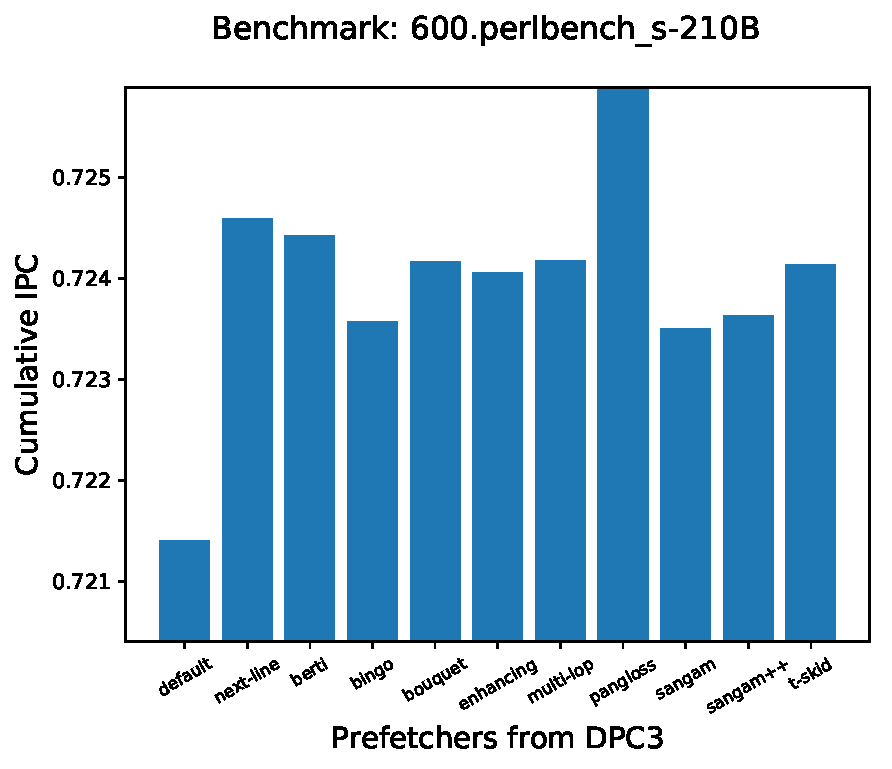
\includegraphics[width=54ex, height=35ex]{600.pdf}
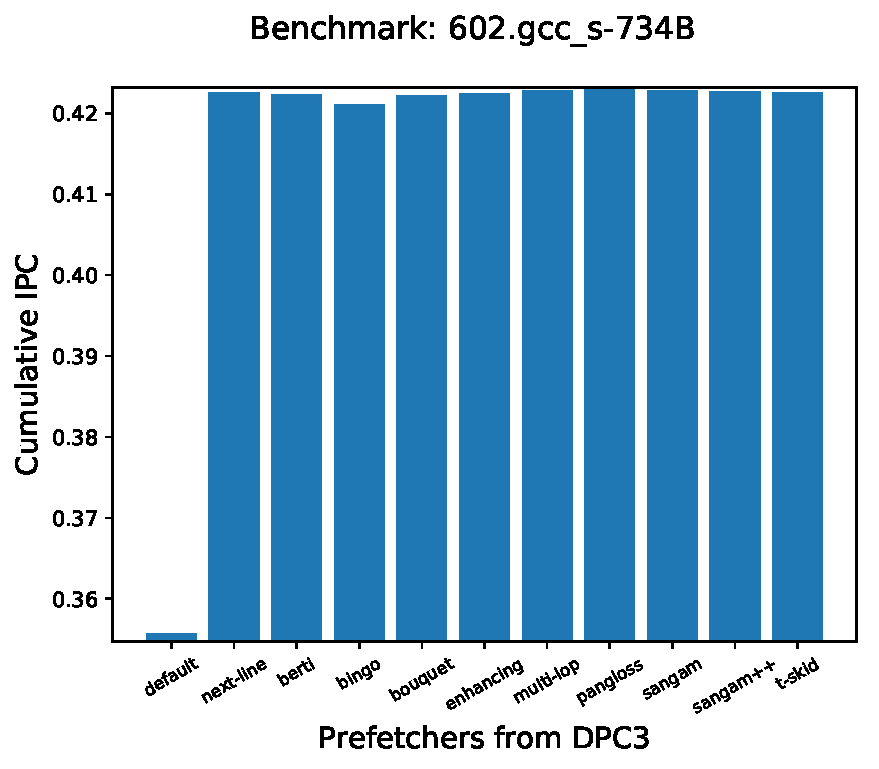
\includegraphics[width=54ex, height=35ex]{602.pdf}
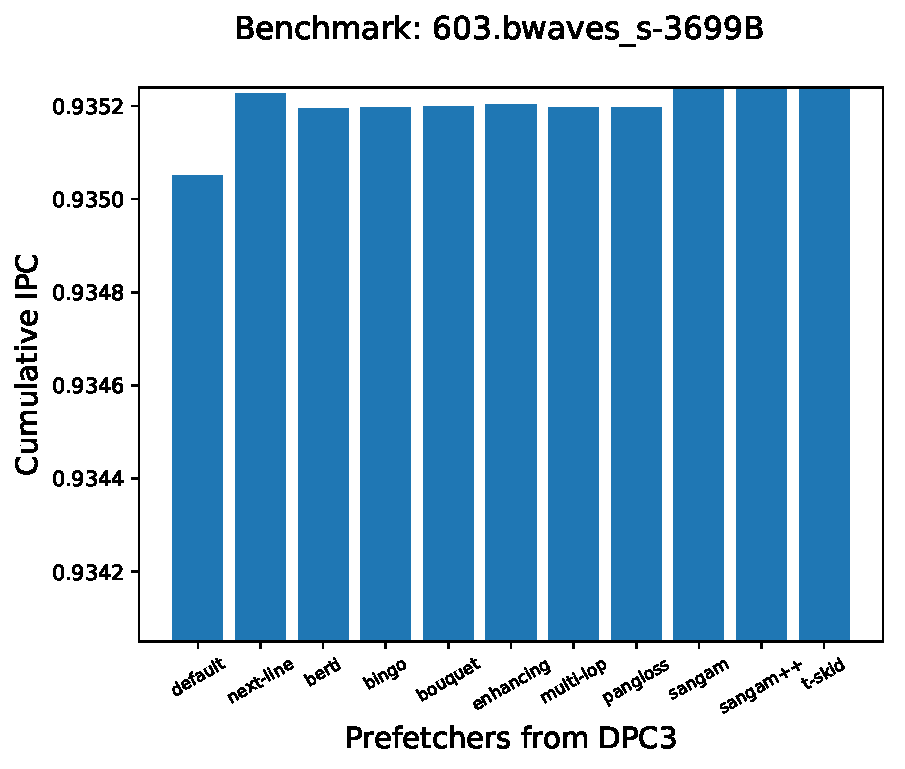
\includegraphics[width=54ex, height=35ex]{603.pdf}
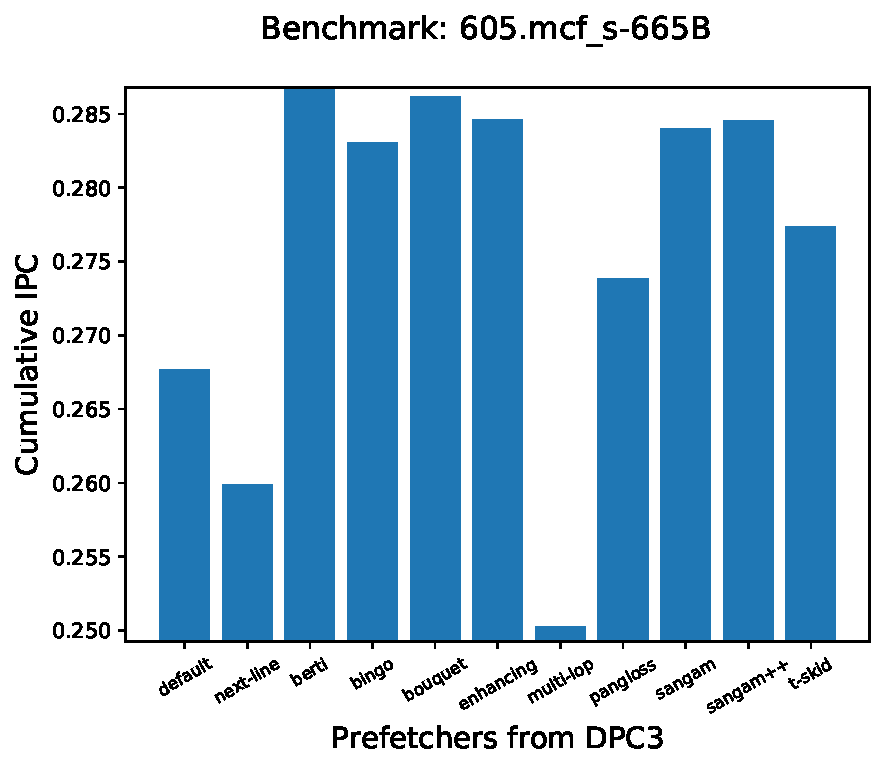
\includegraphics[width=54ex, height=35ex]{605.pdf}
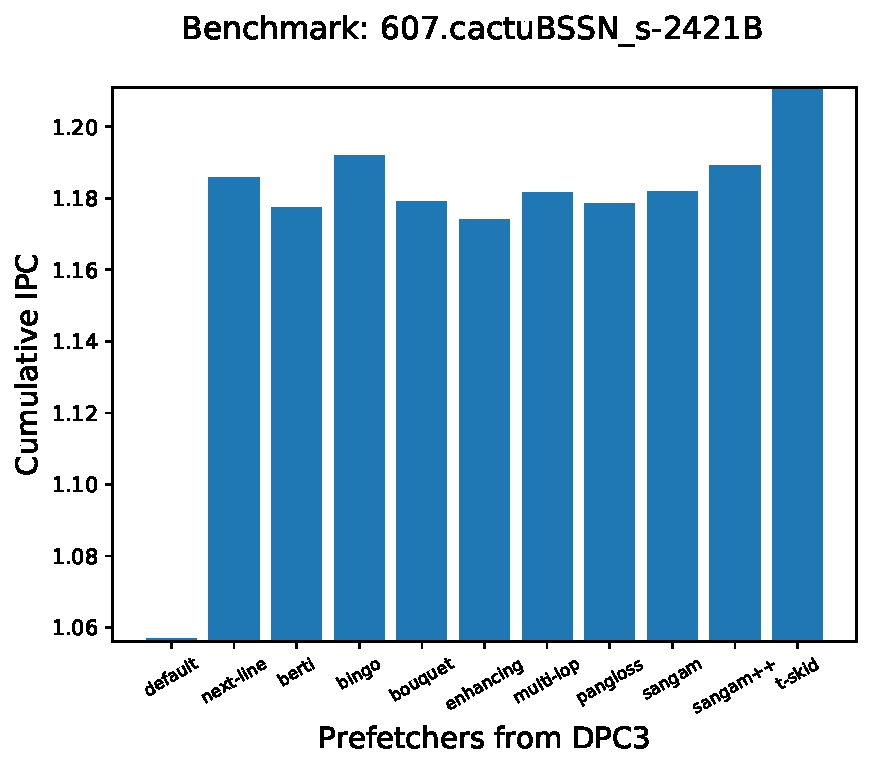
\includegraphics[width=54ex, height=35ex]{607.pdf}
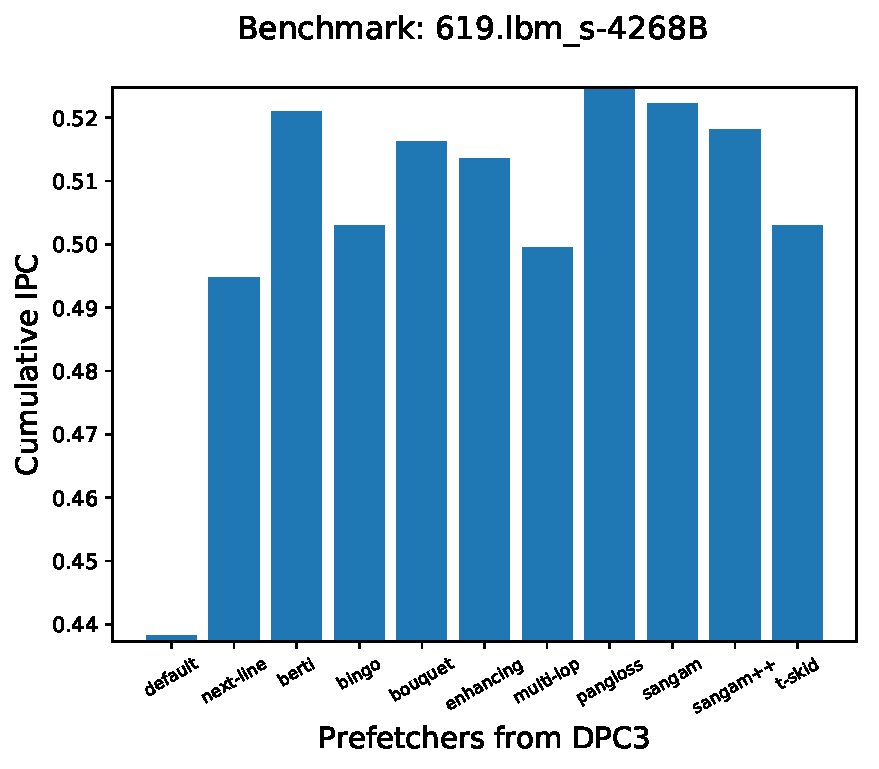
\includegraphics[width=54ex, height=35ex]{619.pdf}
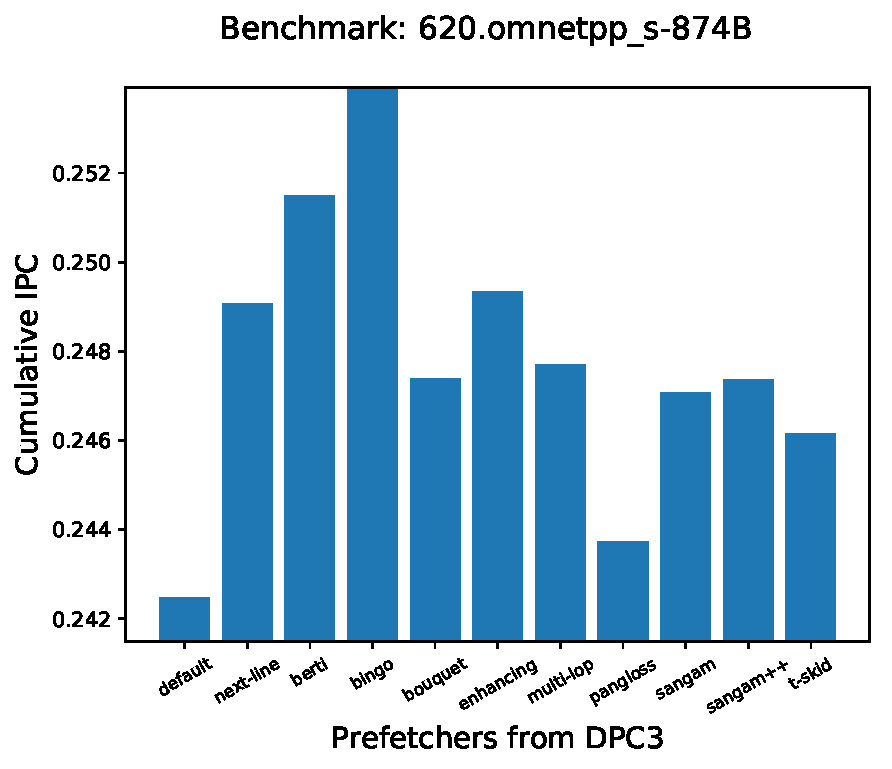
\includegraphics[width=54ex, height=35ex]{620.pdf}
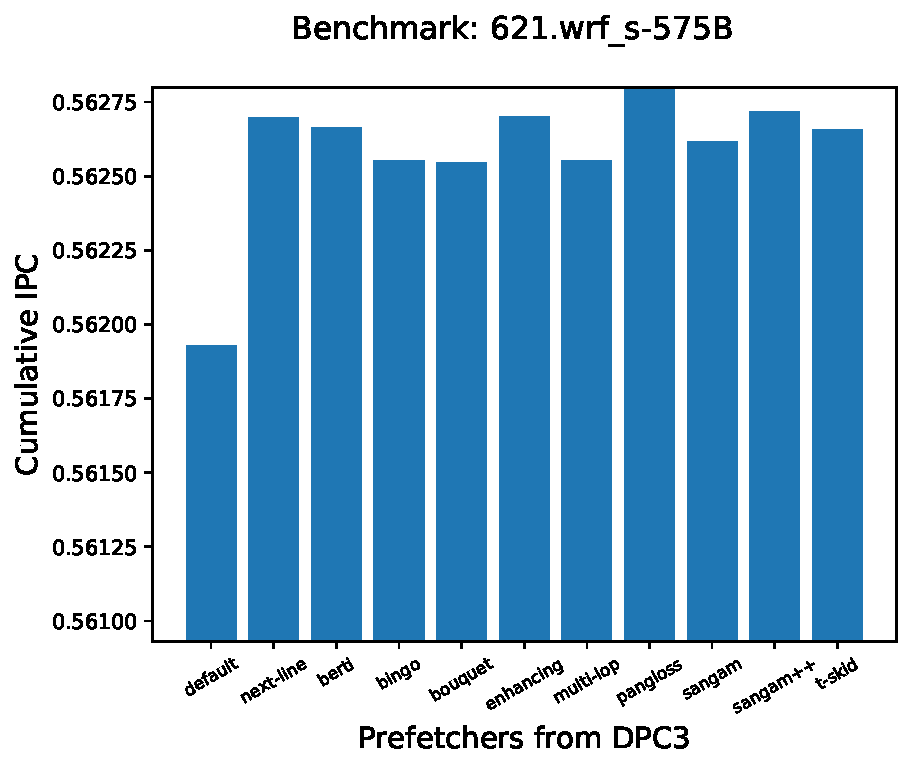
\includegraphics[width=54ex, height=35ex]{621.pdf}
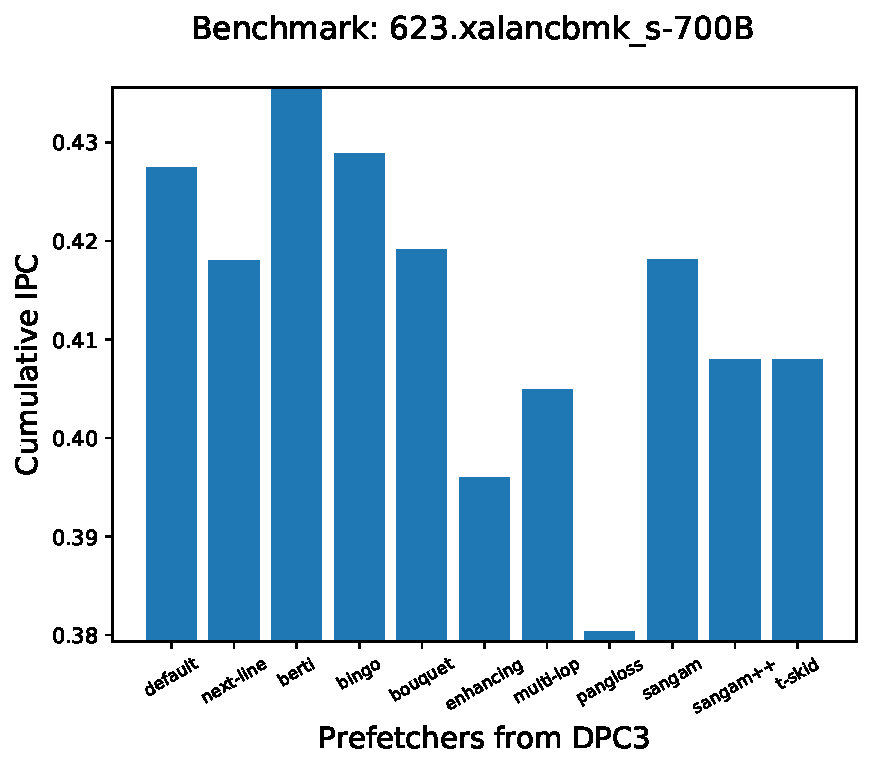
\includegraphics[width=54ex, height=35ex]{623.pdf}
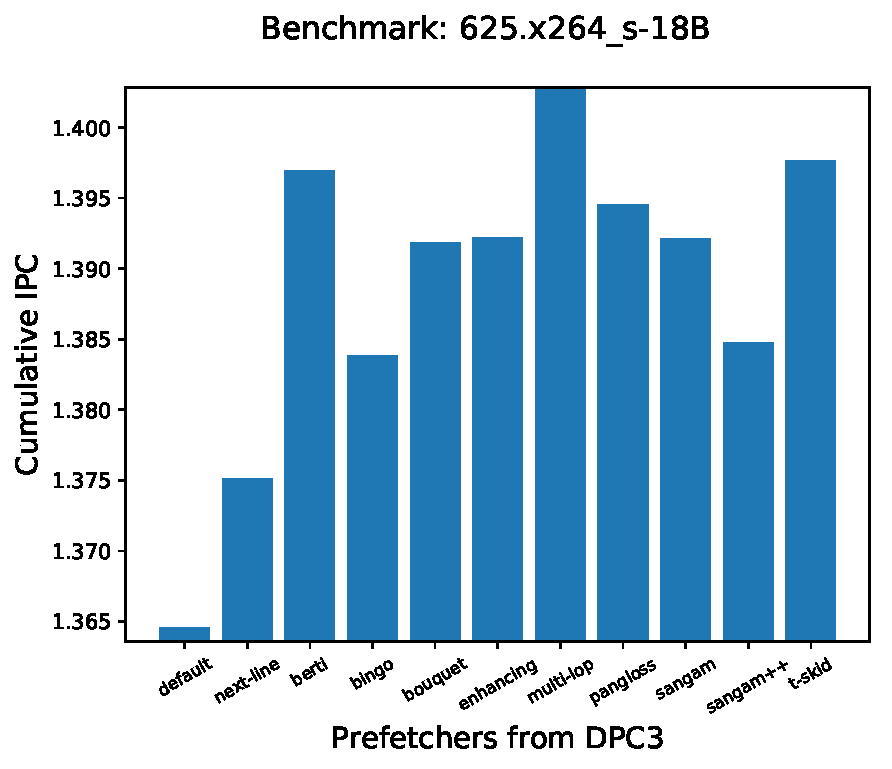
\includegraphics[width=54ex, height=35ex]{625.pdf}
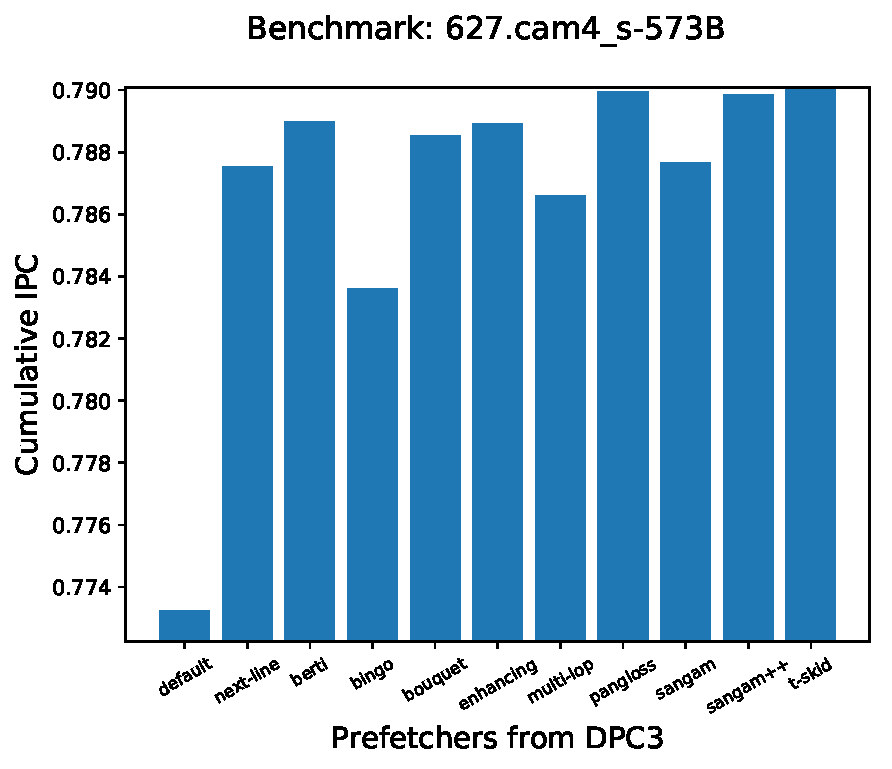
\includegraphics[width=54ex, height=35ex]{627.pdf}
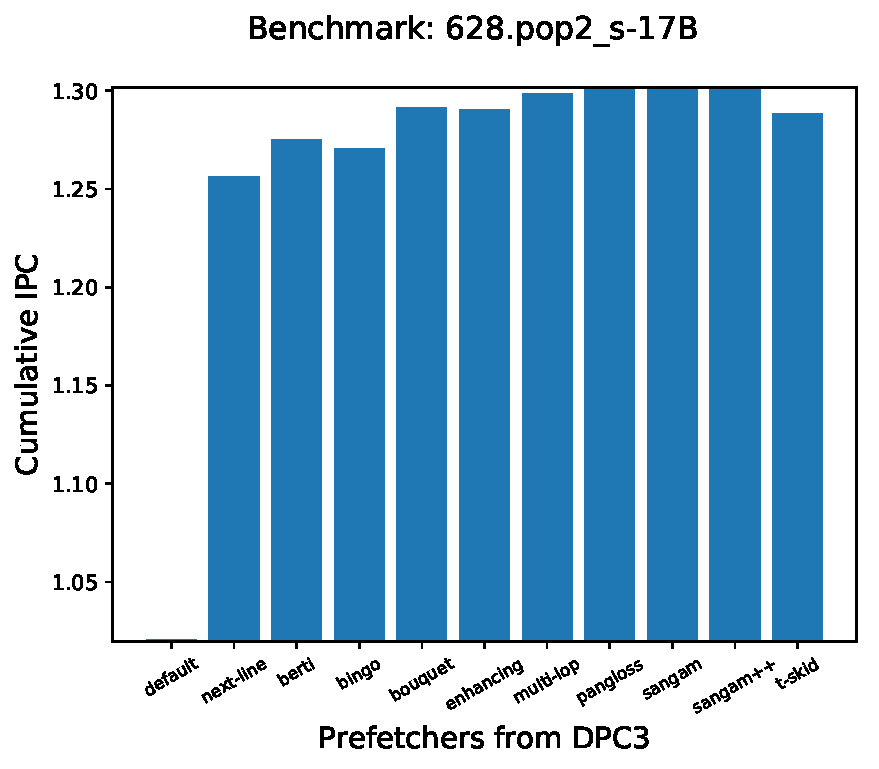
\includegraphics[width=54ex, height=35ex]{628.pdf}
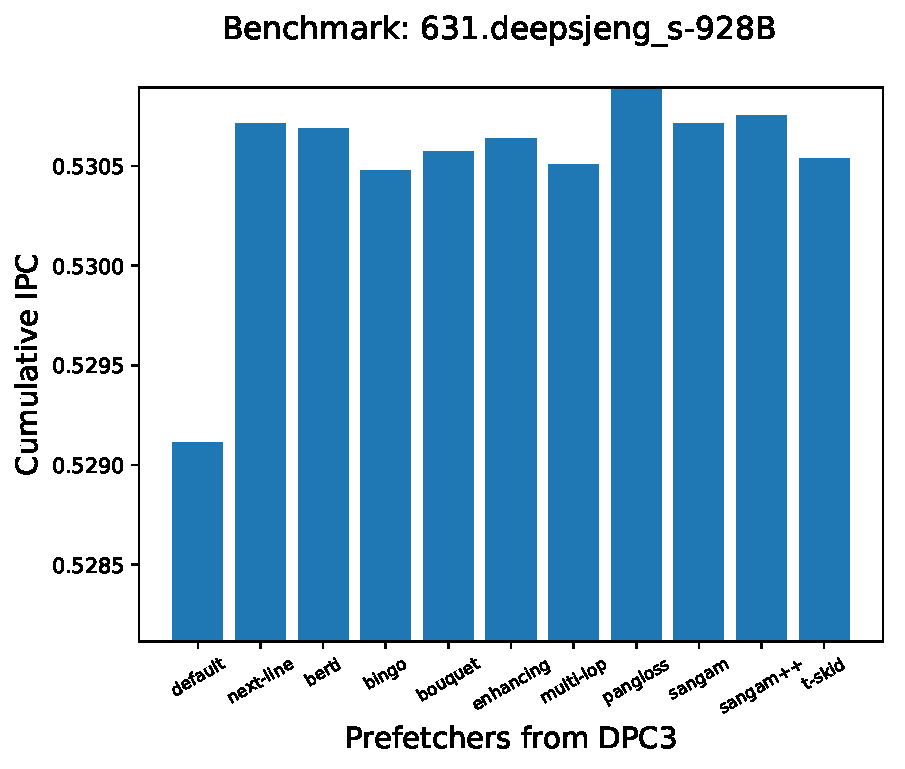
\includegraphics[width=54ex, height=35ex]{631.pdf}
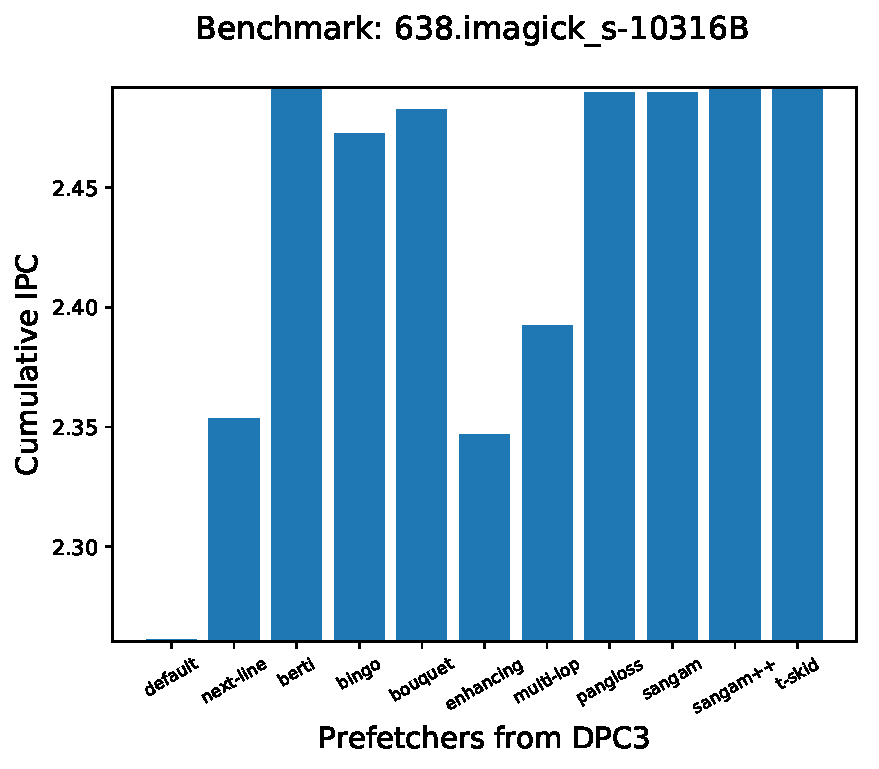
\includegraphics[width=54ex, height=35ex]{638.pdf}
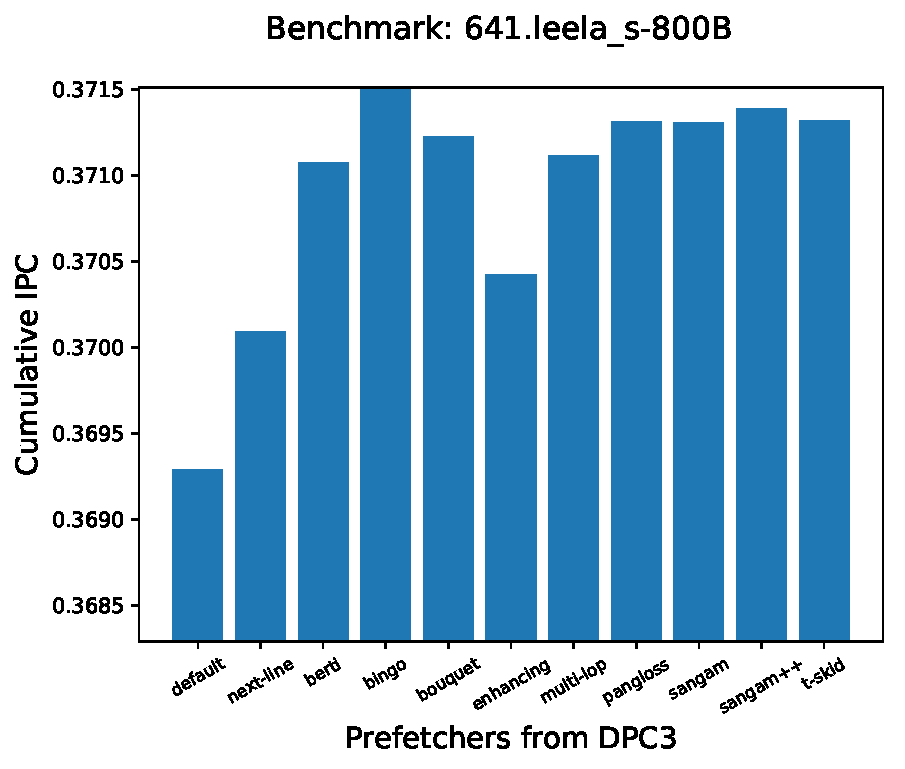
\includegraphics[width=54ex, height=35ex]{641.pdf}
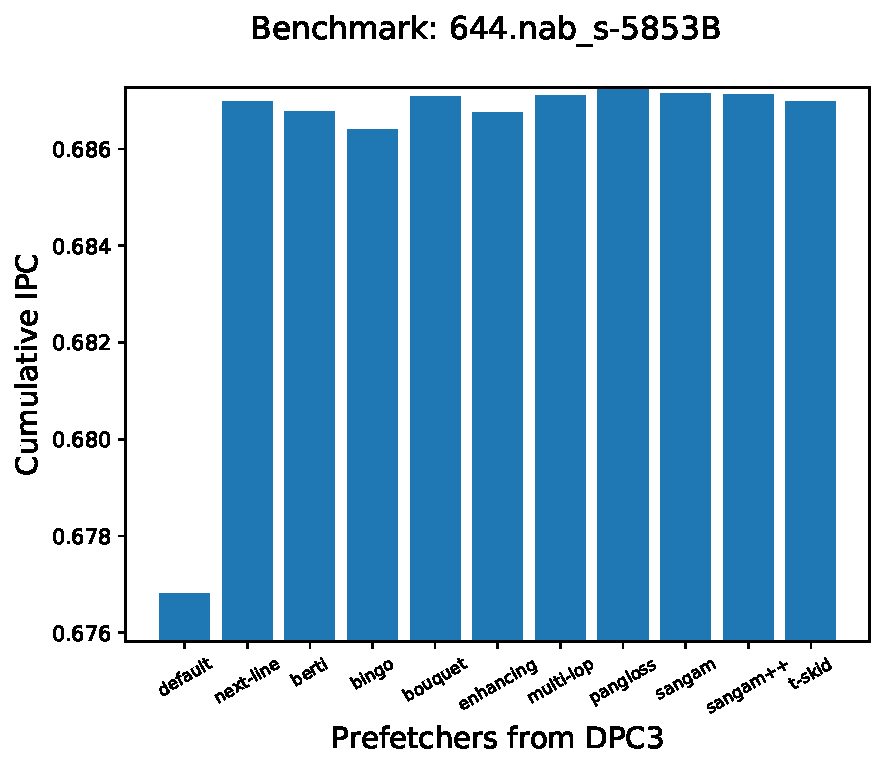
\includegraphics[width=54ex, height=35ex]{644.pdf}
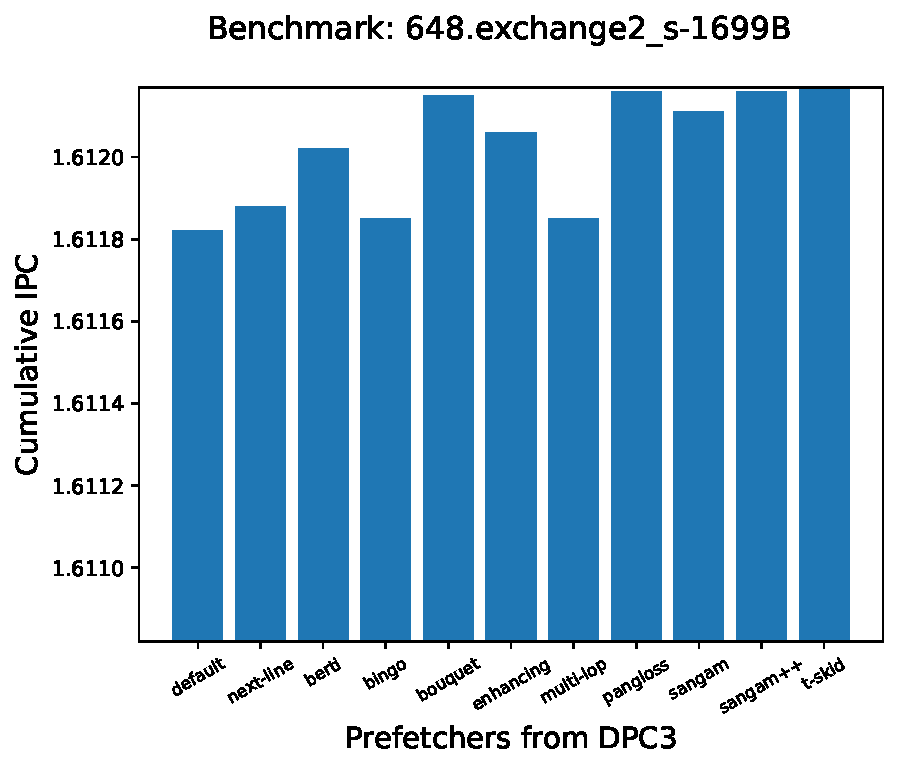
\includegraphics[width=54ex, height=35ex]{648.pdf}
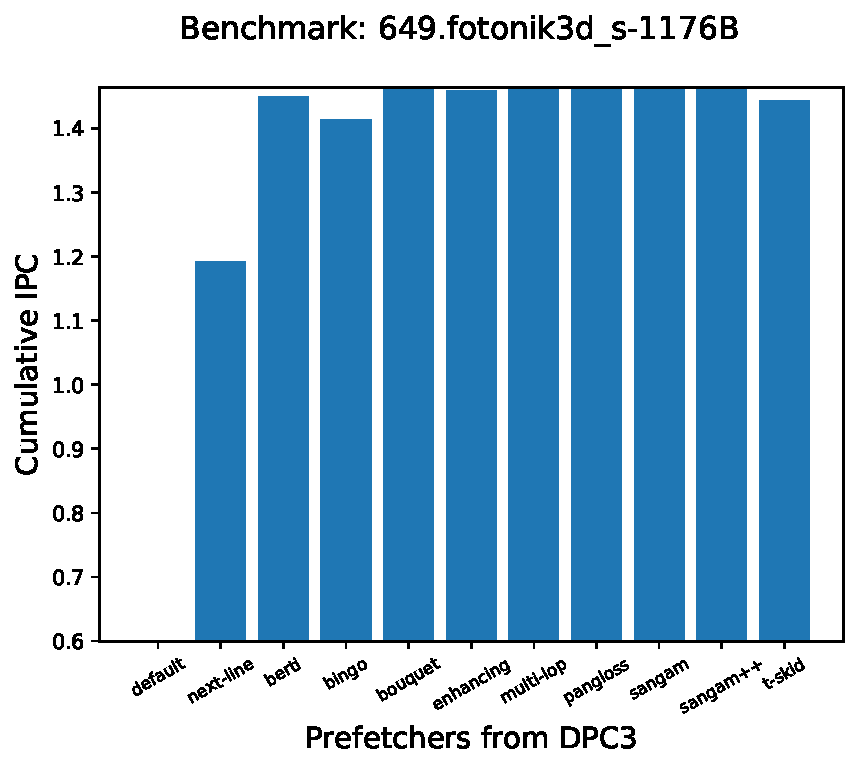
\includegraphics[width=54ex, height=35ex]{649.pdf}
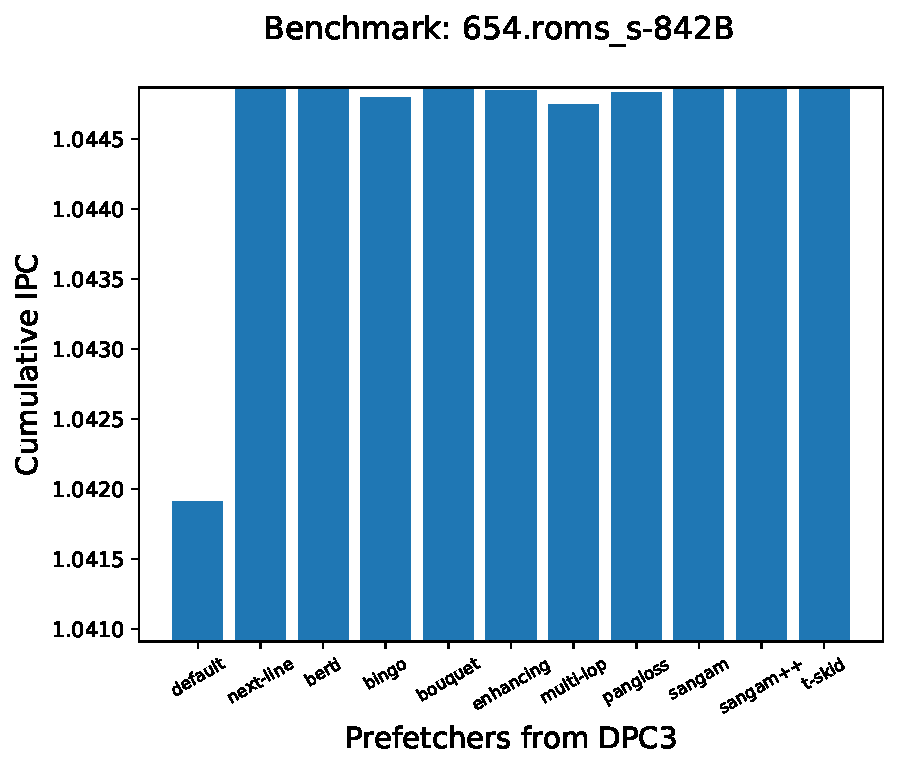
\includegraphics[width=54ex, height=35ex]{654.pdf}
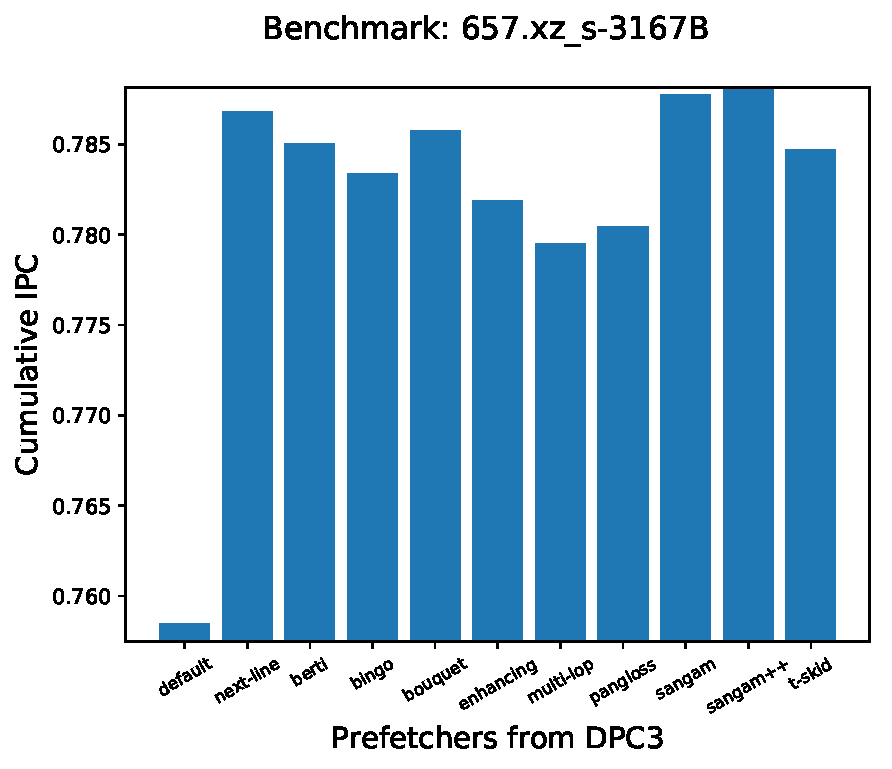
\includegraphics[width=54ex, height=35ex]{657.pdf}

\subsection{Guidelines for Determining Authorship}
IEEE guidelines applete that authorship should be based on a {\em substantial intellectual contribution}. It is assumed that all authors have had a significant role in the creation of an article that bears their names. In particular, the authorship credit must be reserved only for individuals who have met each of the following conditions:

\begin{enumerate}
\item Made a significant intellectual contribution to the theoretical development, system or experimental design, prototype development, and/or the analysis and interpretation of data associated with the work contained in the article;

\item Contributed to drafting the article or reviewing and/or revising it for intellectual content; and

\item Approved the final version of the article as accepted for publication, including references.
\end{enumerate}

A detailed description of the IEEE authorship guidelines and responsibilities is available \href{https://www.ieee.org/publications_standards/publications/rights/Section821.html}{here}. Per these guidelines, it is not acceptable to award {\em honorary } authorship or {\em gift} authorship. Please keep these guidelines in mind while determining the author list of your paper.

\subsection{Declaring Authors}
Declare all the authors of the paper upfront. Addition/removal of authors once the paper is accepted will have to be approved by the program chair, since it potentially undermines the goal of eliminating conflicts for reviewer assignment.

\subsection{Areas and Topics}
Authors should indicate these areas on the submission form as well as specific topics covered by the paper for optimal reviewer match. If you are unsure whether your paper falls within the scope of MICRO, please check with the program chairs -- MICRO is a broad, multidisciplinary conference and encourages new topics.

\subsection{Declaring Conflicts of Interest}
Authors must register all their conflicts on the paper submission site. Conflicts are needed to ensure appropriate assignment of reviewers.  If a paper is found to have an undeclared conflict that causes a problem OR if a paper is found to declare false conflicts in order to abuse or ``game'' the review system, the paper may be rejected. We use the NSF conflict of interest guidelines for determining the conflict period for MICRO 2019.  Please declare a conflict of interest (COI) with the following people for any author of your paper:

\begin{enumerate}
\item Your Ph.D. advisor(s), post-doctoral advisor(s), Ph.D. students,
      and post-doctoral advisees, forever.
\item Family relations by blood or marriage, or their equivalent,
      forever (if they might be potential reviewers).
\item People with whom you have collaborated in the last FOUR years, including:
  \begin{itemize}
  \item co-authors of accepted/rejected/pending papers.
  \item co-PIs on accepted/rejected/pending grant proposals.
  \item funders (decision-makers) of your research grants, and researchers
      whom you fund.
  \end{itemize}
\item People (including students) who shared your primary institution(s) in the
last FOUR years.
\item Other relationships, such as close personal friendship, that you think might tend
to affect your judgment or be seen as doing so by a reasonable person familiar
with the relationship.
\end{enumerate}

``Service'' collaborations such as co-authoring a report for a professional organization, serving on a program committee, or co-presenting  tutorials, do not themselves create a conflict of interest.  Co-authoring a paper that is a compendium of various projects with  no true collaboration among the projects does not constitute a  conflict among the authors of the different projects. On the other hand, there may be others not covered by the above with whom you believe a COI exists, for example, an ongoing collaboration which has not yet resulted in the creation of a paper or proposal. Please report such COIs; however, you may be asked to justify them. Please be reasonable. For example, you cannot declare a COI with a reviewer just because that reviewer works on topics similar to or related to those in your paper.  The PC Chairs may contact co-authors to explain a COI whose origin is unclear.

We hope to draw most reviewers from the PC, but others from the community may also write reviews.  {\bf Please declare all your conflicts (not just restricted to the PC)}.  When in doubt, contact the program chairs.


\subsection{Concurrent Submissions and Workshops}

By submitting a manuscript to MICRO 2019, the authors guarantee that the manuscript has not been previously published or accepted for publication in a substantially similar form in any conference, journal, or the archived proceedings of a workshop (e.g., in the ACM/IEEE digital library) -- see exceptions below. The authors also guarantee that no paper that contains significant overlap with the contributions of the submitted paper will be under review for any other conference or journal or an archived proceedings of a workshop during the MICRO 2019 review period. Violation of any of these conditions will lead to rejection.

The only exceptions to the above rules are for the authors' own papers in (1) workshops without archived proceedings such as in the ACM/IEEE digital library (or where the authors chose not to have their paper appear in the archived proceedings), or (2) venues such as IEEE CAL or arXiv where there is an explicit policy that such publication does not preclude longer conference submissions.  In all such cases, the submitted manuscript may ignore the above work to preserve author anonymity. This information must, however, be provided on the submission form -- the PC chair will make this information available to reviewers if it becomes necessary to ensure a fair review.  As always, if you are in doubt, it is best to contact program chairs.


Finally, the ACM/IEEE Plagiarism Policy (\href{http://www.acm.org/publications/policies/plagiarism_policy}{here} and \href{https://www.ieee.org/publications_standards/publications/rights/plagiarism_FAQ.html}{here}) covers a range of ethical issues concerning the misrepresentation of other works or one's own work.

\section*{Acknowledgements}
This document is derived from previous conferences, in particular MICRO 2013, ASPLOS 2015, MICRO 2015, MICRO 2016, MICRO 2017, and MICRO 2018.


%%%%%%% -- PAPER CONTENT ENDS -- %%%%%%%%


%%%%%%%%% -- BIB STYLE AND FILE -- %%%%%%%%
\bibliographystyle{IEEEtranS}
\bibliography{refs}
%%%%%%%%%%%%%%%%%%%%%%%%%%%%%%%%%%%%

\end{document}
